
\appendixtitle{Coordinate Systems}

\def\Amat\ensuremath{\mathbf{A}}

\subsection{IMU uncertainty}\label{apdx:imu-uncertainty}

\subsection{Measurement frames}\label{apdx:coord-sys:meas}\label{apdx:coord-sys}

\def\a{\ensuremath{\mathrm{a}}}
\def\b{\ensuremath{\mathrm{b}}}
\def\lab{\ensuremath{l_\b^\a}}
\def\xa{\ensuremath{\vec{r}^\a}}
\def\xb{\ensuremath{\vec{r}^\b}}
\def\Rba{\ensuremath{\mathbf{R}^\a_\b}}

Tracking coordinate systems (`reference frames', or simply `frames') is critical to accurately correcting for platform motion of ADV measurements. In general, two three-dimensional, orthogonal, right-handed coordinate systems `a' and `b' are related by the equation:
\begin{align*}
  \xb &= \Rba \cdot (\xa - \lab) & .
\end{align*}
The vectors $\xa$ and $\xb$ point to the same point in space, but in the two distinct coordinate systems.  Superscripts denote the coordinate system that the quantity is measured in and $\cdot$ indicates standard matrix multiplication.  The vector $\lab$ is the `translation vector' that specifies the origin of coordinate system `b' in the `a' frame, and $\mathbf{R}^\mathrm{a}_\mathrm{b}$ is the `orientation matrix' of `b' in `a'. Note that the equation that maps vectors - as opposed to points in space - from one frame to the other does not include $\lab$:
\begin{align}
  \vec{u}^\mathrm{b} & = \Rba \cdot \vec{u}^\mathrm{a}
\end{align}
Also note that for the orthogonal, right-handed coordinate systems considered here the inverse rotation matrix is simply the transpose, $\mathbf{R}^{\mathrm{b}}_{\mathrm{a}}  = (\Rba)^{-1} = (\Rba)^\mathrm{T} $, and the determinant of the rotation matrix is 1, $\mathrm{det}(\Rba ) = 1$.
The coordinate systems for doing so can be broken into two categories: 1) the `inertial' or `stationary' ones into which it is the goal to transform the measurements, and 2) the moving coordinate systems in which sensors make measurements. 

The purpose of this appendix is to clearly document and define the relationships between all of the coordinate systems necessary for quantifying turbulence using moored ADVs.  This appendix starts with general definitions of coordinate systems and the relationships between them (\ref{apdx:coord-sys:math}), then details the stationary and measurement frames used herein (\ref{apdx:coord-sys:stat} and \ref{apdx:coord-sys:meas}, respectively).

\begin{enumerate}
\item the earth reference frame is the inertial coordinate system in
which it is desirable to have measurements of turbulence velocity
\item the IMU reference frame is the reference frame in which that
sensor measures platform motion
\item the ADV-head reference frame is the reference frame in which the
velocity measurements are obtained.
\end{enumerate}

In addition to measuring platform motion the Microstrain IMU provides
an estimate of the orientation of its coordinate system in the earth's
reference frame. Provided that the position and orientation of the
ADV-head is known and fixed in the IMU frame (i.e. they are rigidly
connected), it is possible to estimate the motion of the ADV-head in
the earth reference frame.




\subsection{Defining coordinate systems}\label{apdx:coord-sys:math}


\subsection{The earth frame}
The earth coordinate system is the coordinate system in-which the orientation of the ADV is measured (see \ref{apdx:coord-sys:imu}), and is the coordinate system in-which motion correction is most easily calculated and discussed (section \ref{sec:proc:motion}).  This work utilizes `e' superscripts to denote an `ENU' earth coordinate system with basis vectors,
\begin{itemize}
\item[$\hat{x}\earth$:] East,
\item[$\hat{y}\earth$:] North, and
\item[$\hat{z}\earth$:] Up.
\end{itemize}

\begin{figure}
  \centering
  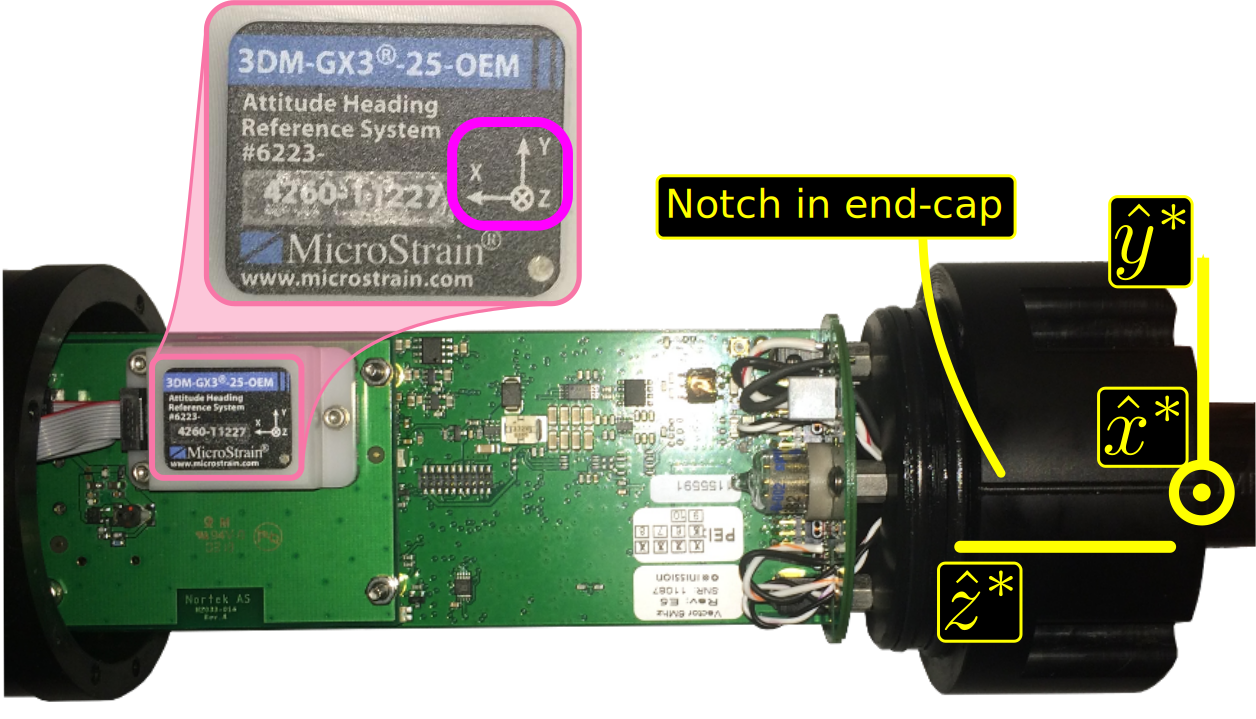
\includegraphics[width=\onewidth]{IMU_Diagram04}
  \caption{The circuit-board and pressure-case end-cap of a Nortek Vector equipped with a Microstrain IMU.  The ADV-body coordinate system (yellow) is depicted on the right. The notch in the end-cap defines the $\hat{x}^*$ direction (out of the page), and the $\hat{z}^*$ direction points back along the pressure case axis. A zoom-in on the Microstrain chip highlights its coordinate system (magenta) relative to the body. }
  \label{fig:imu_orient}
\end{figure}

To combine signals from an IMU with those of an ADV to perform motion correction the coordinate systems in which each of the measurements are made must be carefully accounted for. 

For the Nortek Vector instruments that were used for this work the `ADV-body' coordinate system is defined as being centered on the cylinder-body axis at the point where the head-cable meets its end-cap.  The basis vectors of this coordinate system are defined as (Figures \ref{fig:imu_orient} and \ref{fig:adv-coord-sys}B):
\begin{itemize}
\item[$\hat{x}^*$:] points from the center of the `head' end-cap toward the notch in that end-cap,
\item[$\hat{y}^*$:] is defined by the right-hand-rule based on the other two basis vectors, and
\item[$\hat{z}^*$:] points from the `head' end-cap toward the `battery' end-cap along the body-cylinder (pressure case) axis.
\end{itemize}

\subsubsection{The ADV head}

In order to transform measured velocities into a meaningful reference frame (and to perform motion correction) the orientation (and position) of the ADV head in terms of the body coordinate system must be known. To facilitate this the orientation matrix of the ADV head, $\rmat$, and translation vector\footnote{The position of the ADV-head origin (transmit transducer) in the body coordinate system.}, $\bhv$, are defined according to,
\begin{align}
  \label{eqn:coord_sys}
  \vec{x}^\mathrm{head} &= \rmat \cdot (\vec{x}^* - \bhv) & ,
\end{align}
where $\vec{x}^\mathrm{head}$ and $\vec{x}^*$ are the same point in the head and body coordinate systems, respectively. Combined with the math notes in the previous section, the velocity vectors in the head frame can be transformed into the body frame by,
\begin{align}
  \label{eqn:coord_sys2}
  \vec{u}^* &=  \rmat^\mathrm{T} \cdot \vec{u}^\mathrm{head} & .
\end{align}

For Nortek Vectors, the coordinate system of the ADV head is centered on the transmit transducer face, and the coordinate-directions are defined by (Figure \ref{fig:adv-coord-sys}B, \cite{vector_manual2005}):
\begin{itemize}
\item[$\hat{x}^\mathrm{head}$:] the direction of one of the transducer `receive' arms (marked with tape or paint)
\item[$\hat{y}^\mathrm{head}$:] is defined by the right-hand-rule based on the other two basis vectors, and
\item[$\hat{z}^\mathrm{head}$:] is into the transducer face.
\end{itemize}

For fixed-head Nortek Vector ADVs, the body-frame and head-frame have parallel coordinate systems ($\rmat$ is the identity matrix), and the `head-frame' is translated 21cm along the $z$-axis.  That is, $\bhv = (0, 0, -0.21)$m \cite[]{vector_manual2005}.  

For cable-head ADVs, the position and orientation of the ADV head is arbitrary.  This means that when preparing to make measurements using cable-head ADVs, {\bf the orientation and position of the ADV head must be accurately recorded} in order to allow the ADV measurements to be transformed into the body frame during post-processing. For the example in Figure \ref{fig:adv-coord-sys}A, $\bhv = (254,64,-165)\unit{mm}$, and
\begin{align*}
  \rmat &= \left (
    \begin{array}{ccc}
      0 & 0 & -1 \\
      0 & -1 & 0 \\
      -1 & 0 & 0
    \end{array}
    \right ) & .
\end{align*}
In general $\rmat$ will not necessarily be symmetric nor will it have so many zero-elements (i.e. these characteristics are specific to the head-body alignment of the example).


\begin{figure}
  \centering
  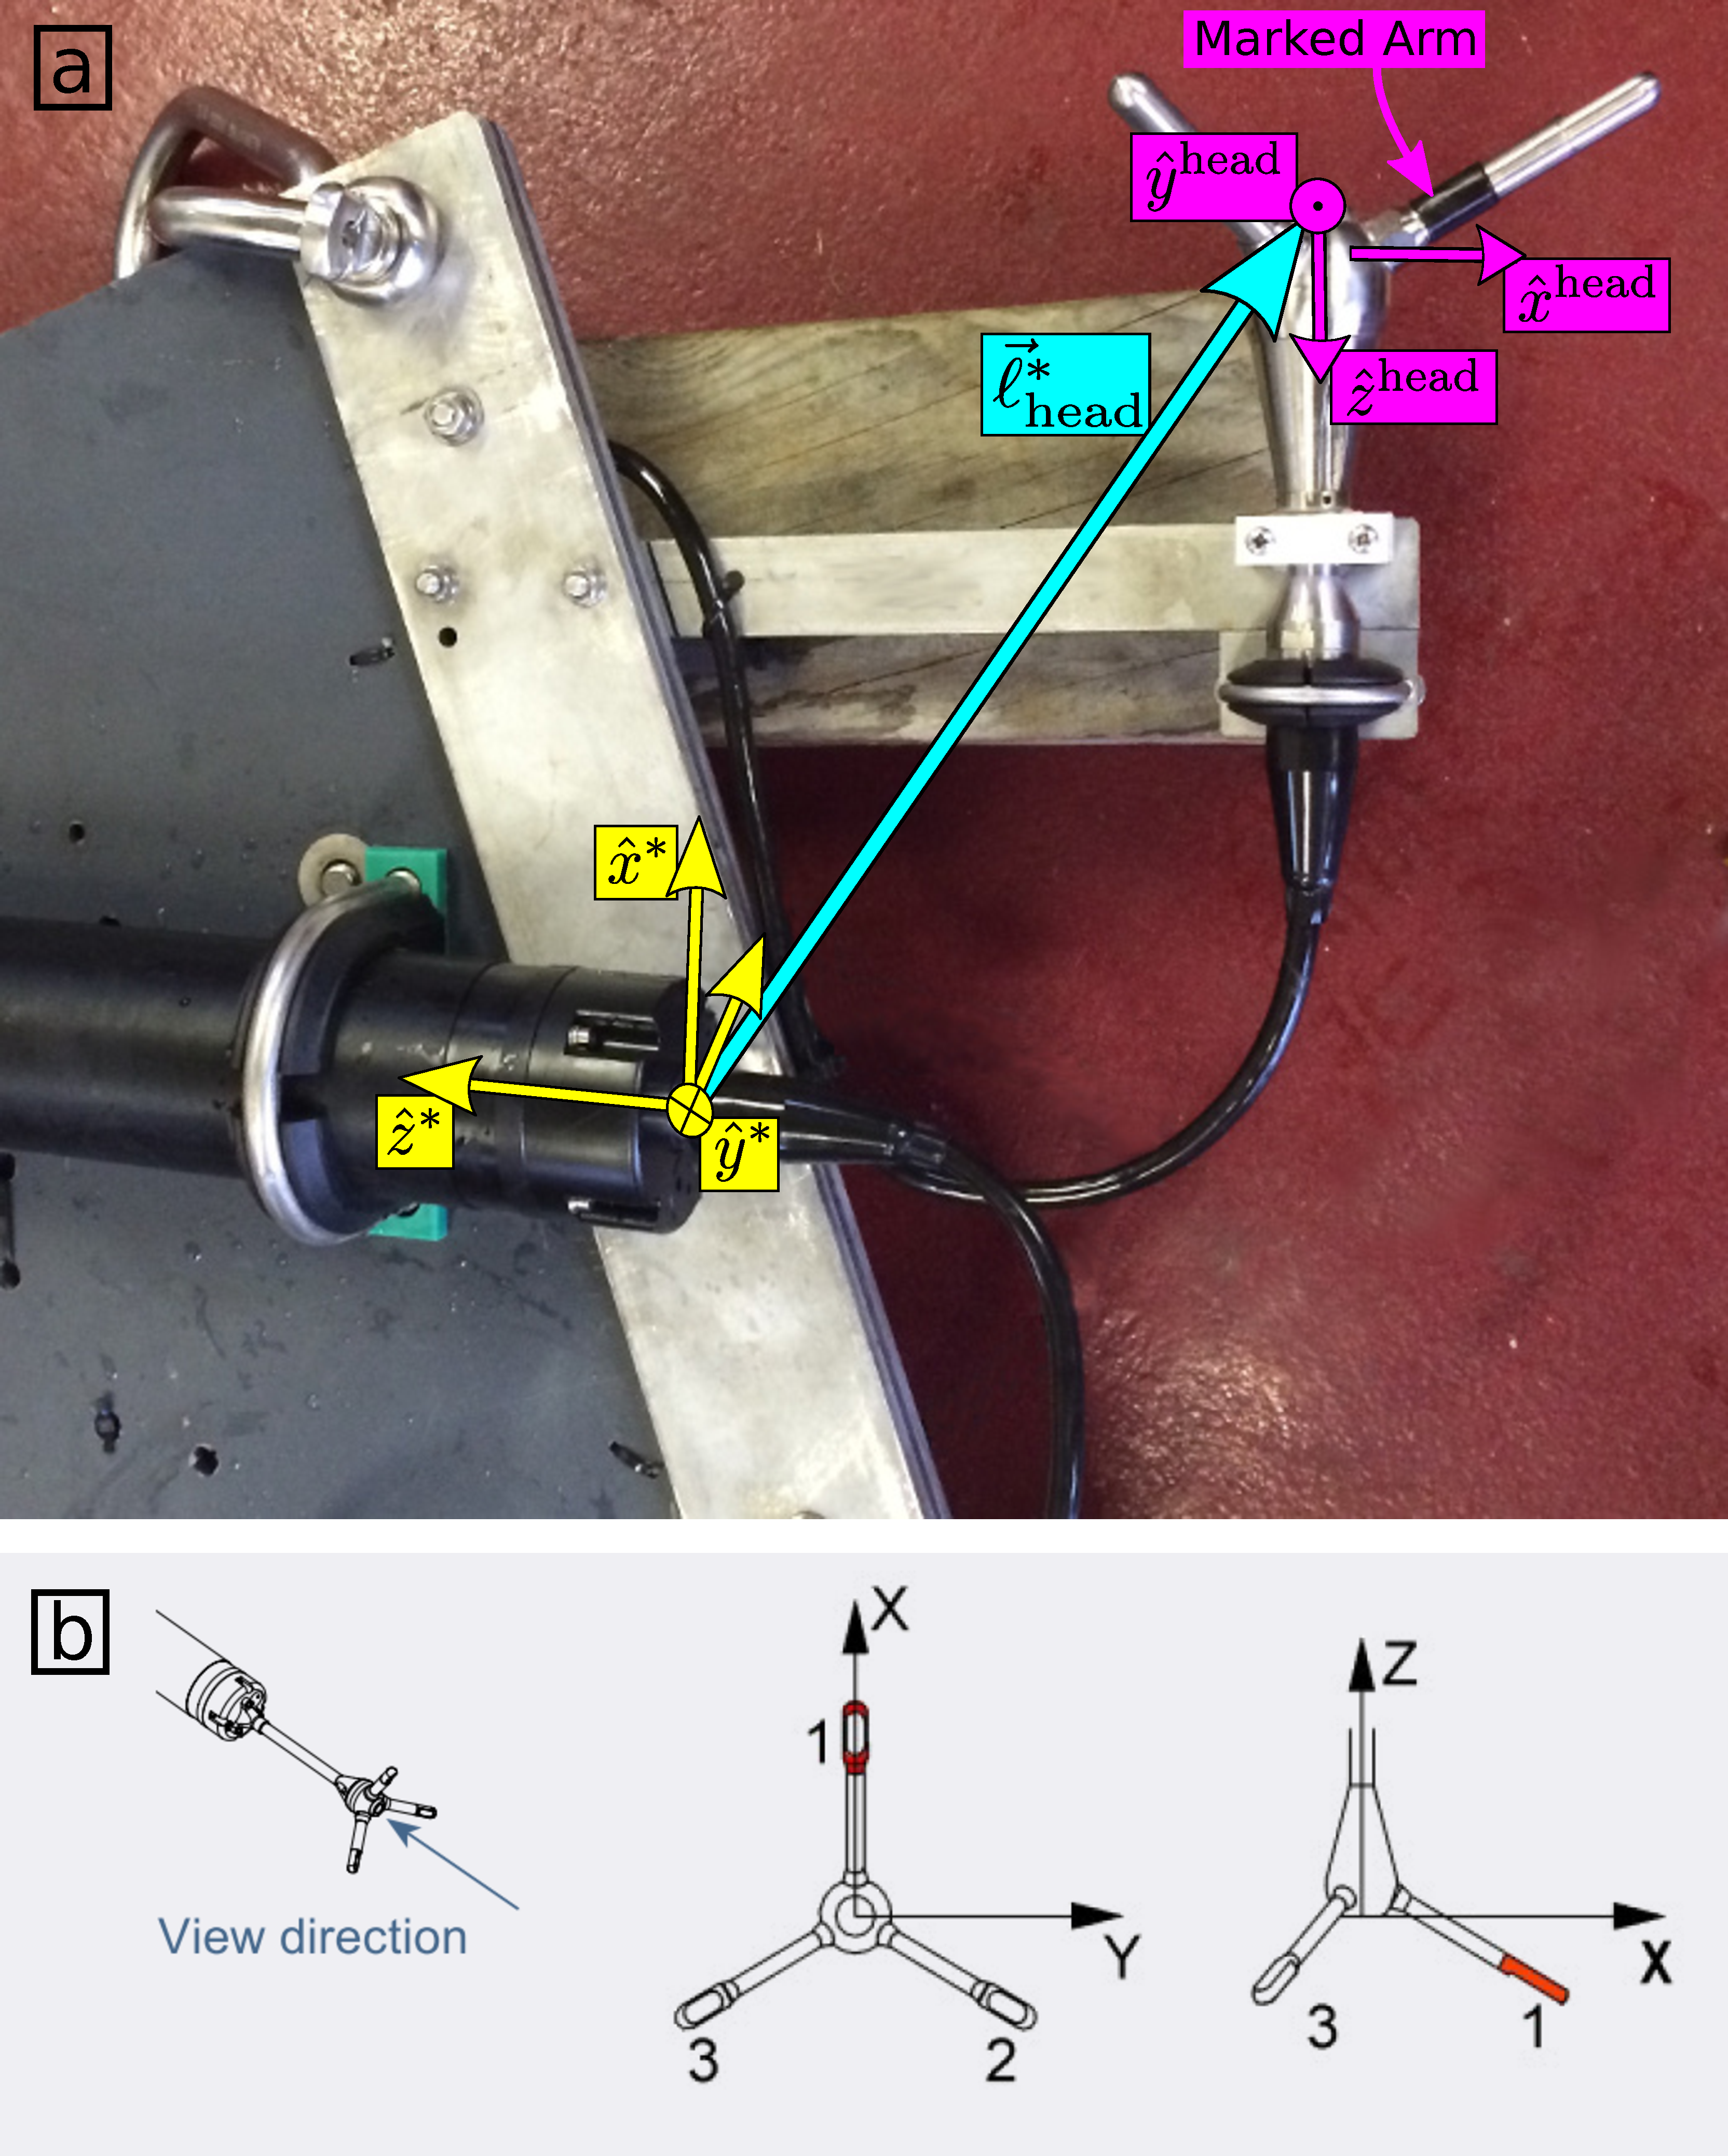
\includegraphics[width=\onewidth]{ADV_coord_sys}
  \caption{Coordinate systems of the ADV body and head. A) A strongback with an ADV rests on a block of wood. Coordinate systems of the ADV head (magenta) and body (yellow) are shown. The $\hat{x}^\mathrm{head}$-direction is known by the black-band around the transducer arm, and the $\hat{x}^*$ direction is marked by a notch on the end-cap (indiscernible in the image). The cyan arrow indicates the body-to-head vector, $\bhv$.  The perspective slightly distorts the fact that  $\hat{x}^\mathrm{head} \parallel -\hat{z}^* $, $\hat{y}^\mathrm{head} \parallel -\hat{y}^* $, and $\hat{z}^\mathrm{head} \parallel -\hat{x}^* $.  B) Coordinate system of the ADV head as defined in the Nortek Vector manual \cite[]{vector_manual2005}. }
  \label{fig:adv-coord-sys}
\end{figure}

\subsubsection{The IMU coordinate system}\label{apdx:coord-sys:imu}

Like the ADV head, the coordinate system in which the IMU measurements are made must be clearly defined and documented. In general, the IMU frame is related to the body coordinate system by,
\begin{align*}
  \vec{x}^\mathrm{imu} &= \mathbf{A}  \cdot (\vec{x}^* - \ihv) & \qquad .
\end{align*}

For the Microstrain 3DM-GX3-25 (IMU) as it is integrated into the Nortek Vector (Figure \ref{fig:imu_orient}), $\ihv = (0.006, 0.006, 0.150)$m and,
\begin{align*}
  \mathbf{A} &=
  \left (
    \begin{array}{ccc}
      0 & 0 & 1 \\
      0 & 1 & 0 \\
      -1 & 0 & 0
    \end{array}
  \right ) & .
\end{align*}


{\bf The orientation matrix}
\def\omatr{\ensuremath{\mathrm{\mathbf{R_\mathrm{imu}}}}}

In order to use the orientation matrix to rotate velocity measurements into an earth-fixed coordinate system it is important to understand how the orientation matrix is defined. The Microstrain IMU outputs an orientation matrix, \omatr, such that:
\begin{align*}
  \vec{u}^\mathrm{imu} & = \omatr \cdot \vec{u}^\mathrm{NED} & .
\end{align*}
Where $\vec{u}^\mathrm{imu}$ and $\vec{u}^\mathrm{NED}$ are vectors in the IMU's local coordinate system and a `north-east-down' (NED) earth-fixed coordinate system, respectively \cite[]{Microstrain2012a}.  
However, this NED earth coordinate system is different from the ENU earth coordinate system used here (and typically used by Nortek \cite[]{nortek_sys_int_manual2011}).  That is,
\begin{align*}
  \vec{u} &= \mathbf{B} \cdot \vec{u}^\mathrm{NED} & ,
\end{align*}
where,
\begin{align*}
  \mathbf{B} & = 
  \left (
    \begin{array}{ccc}
      0 & 1 & 0 \\
      1 & 0 & 0 \\
      0 & 0 & -1
    \end{array}
  \right ) \qquad .
\end{align*}
From this, and the above discussion of the orientation of the IMU in the ADV, it is simple to show that the orientation matrix of the ADV body in a ENU earth frame is,
\begin{align*}
  \omat &= \mathbf{A} \cdot \omatr \cdot \mathbf{B} & ,
\end{align*}
%The \dolfyn\ software package makes this transformation when reading the orientation matrix from Nortek Vector `{\it .vec}' files (i.e. the `orientmat' attribute in the data object returned by \dolfyn .io.read\_nortek is \omat, not \omatr ).  This way vectors in the body frame can be rotated into the ENU earth frame by,
 % \begin{align*}
 %   \vec{u} & = \omatinv \cdot \vec{u}^* & .
 % \end{align*}
